\chapter{Server Benchmarks Tables Results}
\label{chap:appendix-server-benchmarks}
This section provides the reader with the detailed results of the server benchmarks:

\begin{table}[H]
    \centering
    \begin{tabular}{lrrrr}
        \hline
        energy-pkg     & C++                & Go         & PyPy       & Python        \\
        \hline
        1              & 3,756.26            & 28,522.69   & 7,972.65   & \textbf{1,510,534.76}  \\
        2              & 2,591.91            & 18,231.97   & 5,147.60   & 1,141,490.15           \\
        4              & 1,362.61            & 10,304.27   & 2,828.21   &   313,537.85           \\
        8	           &   799.23 	         & 5,617.27    & 1,747.96   &	194,458.98           \\ 
        14             &   603.37            & 3,155.30    & 1,232.03   &   130,506.94           \\
        16             &   627.16            & 2,904.52    & 1,140.80   &   111,438.01           \\
        28             & \textbf{1,830.15}   & 2,306.35    & 1,252.93   &   122,384.40           \\
        28 same CPU    & \textbf{2,116.22}   & 2,271.71    & 1,175.52   &   \textbf{96,049.86}   \\
        32             & \textbf{2,043.31}   & 2,151.74    & 1,257.81   &   120,259.78           \\
        32 same CPU    & \textbf{1,889.55}   & 2,109.37    & 1,155.74   &   \textbf{87,343.61}   \\
        48             &   1,985.14          & 1,856.93    & 1,354.03   &    91,185.55           \\
        60             &   1,975.05          & 1,744.76    & 1,354.03   &    93,015.31           \\
        \hline
    \end{tabular}
\caption[Server - Package energy consumption]{Energy usage by the package on the Server benchmark by implementation and core count}
\label{tab:server-energy-pkg}
\end{table}

\begin{table}[H]
    \centering
    \begin{tabular}{lrrrr}
        \hline
        energy-ram   & C++             & Go                & PyPy                & Python            \\
        \hline      
        1            &   176.83        & 1,049.92          &   355.42            &  59,269.48        \\
        2            &   111.08        &   755.43          &   253.06            &  36,442.43        \\
        4            &    67.60        &   426.69          &   170.08            &  12,799.44        \\
        8	         &    26.28 	   &   175.15          &    88.94            &	  6,683.08       \\
        14           &    18.28        &   107.26          &    72.28            &   4,031.07        \\
        16           &    19.29        &    95.60          &    71.84            &   3,705.32        \\
        28           & 55.09           &    \textbf{55.07} &    \textbf{81.44}   & \textbf{4,057.46} \\
        28 same CPU  & 78.01           &    83.98          &    78.81            &   2,831.52        \\
        32           & 61.70           &    66.51          &    \textbf{83.50}   & \textbf{4,037.98} \\
        32 same CPU  & 65.66           &    66.54          &    77.79            &   2.576.33        \\
        48           & 85.73           &    70.64          &    89.06            &   2,657.54        \\
        60           & 90.01           &    90.23          &    91.31            &   2,703.02        \\
        \hline
    \end{tabular}
\caption[Server - \gls{ram} energy consumption]{Energy usage by the \gls{ram} on the Server benchmark by implementation and core count}
\label{tab:server-energy-ram}
\end{table}

\begin{table}[H]
    \centering
    \begin{tabular}{lrrrr}
        \hline
        time         & C++             & Go            & PyPy          & Python     \\
        \hline
        1            & 23.70           & 172.952       & 46.58         & 5,913.41        \\
        2            & 12.52           & 89.32         & 26.43         & 4,749.55        \\
        4            & 6.69            & 45.51         & 13.97         & 1,665.41        \\
        8	         & 3.51  	       & 23.78 	       & 7.66          & 872.89          \\
        14           & 2.39            & 14.03         & 5.15          & 528.12          \\
        16           & 2.55            & 12.46         & 4.88          & 482.30          \\
        28           & 11.63           & 8.91          & 5.39          & 529.22          \\
        28 same CPU  & 13.82           & 7.61          & 3.77          & 269.13          \\
        32           & 8.39            & 8.16          & 5.44          & 523.04          \\
        32 same CPU  & 11.85           & 6.82          & 3.58          & \textbf{244.57} \\
        48           & 15.46           & 6.82          & 4.03          & 252.17          \\
        60           & 15.94           & \textbf{5.36} & \textbf{4.05} & 256.87          \\
        \hline
    \end{tabular}
\caption[Server - Execution Time]{Execution time on the Server benchmark by implementation and core count}
\label{tab:server-execution-time}
\end{table}

\chapter{Desktop Tables Results}
\label{chap:appendix-desktop-benchmarks}

This section provides the reader with the detailed results of the personal desktop benchmarks, including energy consumption, RAM power consumption and execution times for the benchmarks ran on a personal desktop with different core counts and programming languages.

\begin{table}[H]
 \centering
    \begin{tabular}{lrrrr}
    \hline
    energy-pkg & C++ & Go & PyPy & Python \\
    \hline
    1 & 991.49 & 5,867.26 & 1,621.77 & 272,235.58 \\
    2 & 657.79 & 3,746.84 & 1,324.05 & 174,822.21 \\
    4 & 442.17 & 2,335.54 & 938.02 & 112,247.92 \\
    8 & 354.57 & 1,583.17 & 747.41 & 82,983.52 \\
    12 & 339.44 & 1,324.22 & 842.68 & 90,069.44 \\
    14 & 333.01 & 1,247.80 & 889.03 & 93,771.09 \\
    16 & 321.60 & 1,194.03 & 937.02 & 98,436.51 \\
    \hline
    \end{tabular}
\caption[Desktop - Package energy consumption with Hyperthreading]{Energy usage by the package on the Desktop benchmark by implementation and core count with Hyperthreading enabled}
\label{tab:desktop-energy-pkg-hyperthreading}
\end{table}

\begin{table}[H]
    \centering
    \begin{tabular}{lrrrr}
        \hline
        energy-pkg     & C++                 & Go          & PyPy       & Python              \\
        \hline
        1              & 1,008.55            & 5,945.33    & 1,635.95   &                    \\
        2              & 671.13              & 3,652.85    & 1,296.42   & 176,092.08         \\
        4              & 437.34              & 2,421.40    & 914.60     & 113,582.17         \\
        6              & 388.96              & 1,878.72    & 789.89     & 95,214.00          \\
        8	           & 346.15              & 1,645.18    & 735.35     & 82,869.55          \\
        \hline
    \end{tabular}
\caption[Desktop - Package energy consumption]{Energy usage by the package on the Desktop benchmark by implementation and core count}
\label{tab:desktop-energy-pkg}
\end{table}

TODO:
Esto está en esta gráfica: \autoref{fig:log-desktop-energy-pkg} y \autoref{fig:linear-desktop-energy-pkg}, hay un benchmark que no está bien del desktop, 4 cores.

\begin{table}[H]
 \centering
    \begin{tabular}{lrrrr}
    \hline
    execution-time & C++ & Go & PyPy & Python \\
    \hline
    1 & 22.78 & 178.98 & 37.12 & 6,063.96 \\
    2 & 11.71 & 70.51 & 21.62 & 3,084.07 \\
    4 & 6.23 & 36.79 & 12.28 & 1,600.72 \\
    8 & 3.45 & 19.18 & 6.85 & 825.24 \\
    12 & 3.20 & 14.33 & 6.95 & 848.99 \\
    14 & 3.09 & 12.97 & 7.01 & 866.47 \\
    16 & 2.97 & 12.09 & 7.21 & 878.90 \\
    \hline
    \end{tabular}
\caption[Desktop - Execution Time with Hyperthreading]{Execution time on the Desktop benchmark by implementation and core count with Hyperthreading enabled}
\label{tab:desktop-execution-time-hyperthreading}
\end{table}

\begin{table}[H]
    \centering
    \begin{tabular}{lrrrr}
        \hline
        execution-time & C++                 & Go          & PyPy       & Python              \\
        \hline
        1              & 22.60               & 178.43      & 36.42      &                    \\
        2              & 11.64               & 69.77       & 21.59      & 3,115.45           \\
        4              & 6.20                & 36.68       & 11.97      & 1,634.00           \\
        6              & 4.49                & 25.24       & 8.35       & 1,104.04           \\
        8	           & 3.43                & 20.84       & 6.91       & 829.50             \\
        \hline
    \end{tabular}
\caption[Desktop - Execution Time]{Execution time on the Desktop benchmark by implementation and core count}
\label{tab:desktop-execution-time}
\end{table}

\chapter{Laptop Benchmarks Tables Results}
\label{chap:appendix-laptop-benchmarks}

This section provides the reader with the detailed results of the laptop benchmarks, including energy consumption and execution times for the benchmarks ran on a MacBook Pro with different core counts and programming languages.

\begin{table}[H]
    \centering
    \begin{tabular}{lrrrr}
        \hline
        Cores & C++   & Go       & PyPy 3.11.11 & Python      \\
        \hline
        1     & 58.79  & 429.23  & 194.69       & 17,546.05   \\
        2     & 68.93  & 370.01  & 211.21       & 16,322.57   \\
        4     & 54.97  & 354.64  & 216.53       & 16,193.99   \\
        8     & 55.94  & 348.14  & 216.60       & 15,509.12   \\
        10    & 55.00  & 336.88  & 214.96       & 14,942.09   \\
        14    & 48.39  & 300.66  & 203.92       & 13,777.34   \\
        \hline
    \end{tabular}
\caption[Laptop - Package energy consumption]{Energy usage by the package on the Laptop benchmark by implementation and core count}
\label{tab:mbp-power-consumption}
\end{table}

\begin{table}[H]
    \centering
    \begin{tabular}{lrrrr}
        \hline
        Cores & C++  & Go    & PyPy 3.11.11 & Python    \\
        \hline
        1     & 7.48  & 54.16  & 26.52        & 2,697.08  \\
        2     & 3.63  & 26.76  & 15.55        & 1,356.76  \\
        4     & 2.06  & 14.80  & 8.25         & 696.75    \\
        8     & 1.37  & 7.94   & 4.57         & 350.76    \\
        10    & 1.26  & 6.66   & 3.81         & 288.37    \\
        14    & 1.48  & 5.94   & 3.62         & 262.00    \\
        \hline
    \end{tabular}
\caption[Laptop - Execution Time]{Execution time on the Laptop benchmark by implementation and core count}
\label{tab:mbp-time-execution}
\end{table}


\chapter{Raspberry Pi Benchmarks Tables Results}
\label{chap:appendix-rpi-benchmarks}

This section provides the reader with the detailed results of the Raspberry Pi benchmarks, including energy consumption and execution times for the benchmarks ran on a Raspberry Pi 5 with different core counts and programming languages.

\begin{table}[h]
    \centering
    \begin{tabular}{lrrrr}
        \hline
        Cores & C++    & Go      & PyPy         & Python      \\
        \hline
        1     & 80.00  & 236.67  & 190.00       & 11\,780.00  \\
        2     & 51.67  & 153.33  & 152.33       &  7\,620.67  \\
        4     & 41.28  & 107.20  & 181.60       &  5\,739.00  \\
        \hline
    \end{tabular}
\caption[Raspberry Pi - Package energy consumption]{Energy usage by the package on the Raspberry Pi benchmark by implementation and core count}
\label{tab:rpi-power-consumption}
\end{table}

\begin{table}[H]
    \centering
    \begin{tabular}{lrrrr}
        \hline
        Cores & C++    & Go      & PyPy         & Python      \\
        \hline
        1     & 49.26  & 165.03  & 126.36       & 8\,853.08   \\
        2     & 25.25  &  81.98  &  74.42       & 4\,423.91   \\
        4     & 12.80  &  41.10  &  72.14       & 2\,264.50   \\
        \hline
    \end{tabular}
\caption[Raspberry Pi - Execution Time]{Execution time on the Raspberry Pi benchmark by implementation and core count}
\label{tab:rpi-time-execution}
\end{table}

\chapter{Goroutines Benchmarks}
\begin{table}
  \centering
  \begin{tabular}{lcrcrc}
    \toprule
    Cores & Goroutines & Energy (J) & Relative Energy & Execution time (s) & Relative Time \\
    \midrule
    1             & 1          &  28,522.69         & $1x$              &  172.952          &  $1x$               \\
    1             & 2          &  28,919.31         & $0.99x$           &  175.381          &  $0.99x$            \\
    2             & 2          &  18,231.97         & $1.56x$           &   89.319          &  $1.94x$            \\
    2             & 4          &  18,224.50         & $1.57x$           &   89.275          &  $1.94x$            \\
    4             & 4          &  10,304.27         & $2.77x$           &   45.508          &  $3.8x$             \\
    4             & 8          &  10,299.06         & $2.77x$           &   45.482          &  $3.8x$             \\
    8             & 8          &  \textbf{5,617.27} & \textbf{$5.08x$}  &   \textbf{23.781} &  \textbf{$7.27x$}   \\
    8             & 16         &  5,580.52          & $5.11x$           &   23.594          &  $7.33x$            \\
    14            & 14         &  3,155.30          & $9.04x$           &   14.034          &  $12.32x$           \\
    14            & 28         &  3,151.93          & $9.05x$           &   14.001          &  $12.35x$           \\
    16            & 16         &  2,904.52          & $9.82x$           &   12.456          &  $13.88x$           \\
    16            & 32         &  3,018.54          & $9.45x$           &   12.435          &  $13.91x$           \\
    28            & 28         &  2,306.35          & $12.37x$          &    8.906          &  $19.42x$           \\
    28 \textbf{*} & 28         &  \textbf{2,271.71} & \textbf{$12.56x$} &    \textbf{7.613} &  \textbf{$22.72x$}  \\
    28            & 56         &  2,314.29          & $12.32x$          &    7.791          &  $22.2x$            \\
    28 \textbf{*} & 56         &  \textbf{2,290.85} & \textbf{$12.45x$} &    \textbf{8.815} &  \textbf{$19.62x$}  \\
    32            & 32         &  2,151.74          & $13.26x$          &    8.163          &  $21.19x$           \\
    32 \textbf{*} & 32         &  \textbf{2,109.37} & \textbf{$13.52x$} &    \textbf{6.822} &  \textbf{$25.35x$}  \\
    32            & 64         &  2,121.88          & $13.44x$          &    8.101          &  $21.35x$           \\
    32 \textbf{*} & 64         &  \textbf{2,142.21} & \textbf{$13.31x$} &    \textbf{6.896} &  \textbf{$25.08x$}  \\
    48            & 48         &  1,856.93          & $15.36x$          &    5.718          &  $30.24x$           \\
    48            & 96         &  1,848.47          & $15.43x$          &    5.673          &  $30.48x$           \\
    60            & 60         &  1,744.76          & $16.35x$          &    5.357          &  $32.28x$           \\
    60            & 120        &  1,737.80          & $16.41x$          &    5.320          &  $32.5x$            \\
    60            & 200        &  1,724.73          & $16.54x$          &    5.255          &  $32.91x$           \\
    60            & 250        &  1,719.49          & $16.59x$          &    5.218          &  $33.14x$           \\
    \bottomrule
  \end{tabular}
  \caption[Go goroutines and cores]{Go goroutines and cores used, \textbf{*} means the execution is fixed to one CPU}
  \label{tab:go-routines-cores}
\end{table}

\chapter{Compiler Optimizations Tables Results}
\begin{table}
  \centering
  \caption{Power/Energy and execution time for various core counts and compiler optimization flags}
  \label{tab:compiler-optimizations}
  \begin{tabular}{lrrrrr}
    \toprule
    \textbf{Metric / Flags} & \textbf{-O0} & \textbf{-O1} & \textbf{-O2} & \textbf{-O3} & \textbf{-O3 (fast-math)} \\
    \midrule
    \multicolumn{6}{c}{\textbf{1 core}} \\
    power/energy-pkg (J) & 52,957.47 & 5,185.28 & 4,388.12 &  4,031.83   & \textbf{4,005.70} \\
    power/energy-ram (J) & 2,208.08  & 210.28   & 183.21   &    180.00   & \textbf{168.52}  \\
    time (s)             & 270.06    & 27.453   & 24.02    &     23.5993 & \textbf{22.054}  \\
    \midrule
    \multicolumn{6}{c}{\textbf{4 cores}} \\
    power/energy-pkg (J) & 13,379.59 & 1,564.51 & 1,417.01 & \textbf{1,386.60} & 1,414.08       \\
    power/energy-ram (J) & 508.40    & 56.72    & 50.96    &     50.37         & \textbf{49.56}  \\
    time (s)             & 66.066    & 7.4351   & 6.67     &    6.5605         & \textbf{6.478}  \\
    \midrule
    \multicolumn{6}{c}{\textbf{14 cores}} \\
    power/energy-pkg (J) & 5,056.15  & 658.46   & 606.58   & \textbf{595.29}  & 639.00         \\
    power/energy-ram (J) & 153.03    & 20.79    & 18.53    & \textbf{18.24}  & 20.10          \\
    time (s)             & 19.9344   & 2.7184   & 2.42     & \textbf{2.3807} & 2.62           \\
    \midrule
    \multicolumn{6}{c}{\textbf{28 cores}} \\
    power/energy-pkg (J) & 3,650.43  & 627.89   & 565.83   &    561.59   & \textbf{547.56} \\
    power/energy-ram (J) & 120.49    & 20.00    & 18.00    &     17.93   & \textbf{17.47}  \\
    time (s)             & 15.729    & 2.6043   & 2.36     &     2.3382  & \textbf{2.2701} \\
    \midrule
    \multicolumn{6}{c}{\textbf{32 cores}} \\
    power/energy-pkg (J) & 3,353.53  & 606.52   & 552.98   &     548.83  & \textbf{535.22} \\
    power/energy-ram (J) & 110.47    & 19.54    & 17.76    &     17.58   & \textbf{17.27}  \\
    time (s)             & 14.4472   & 2.5369   & 2.33     &     2.3015  & \textbf{2.2368} \\
    \midrule
    \multicolumn{6}{c}{\textbf{60 cores}} \\
    power/energy-pkg (J) & 2,794.03  & 698.96   & 661.76   & \textbf{659.31} & 671.51         \\
    power/energy-ram (J) & 86.80     & 25.37    & 24.11    & \textbf{24.10}  & 24.76          \\
    time (s)             & 7.5463    & 1.89955  & 1.80     &     1.79288     & \textbf{1.79288}\\
    \bottomrule
  \end{tabular}
\end{table}

\chapter{Number of Benchmarks for average calculation}
\label{chap:appendix-number-benchmarks}

The number of benchmarks that are run for each of the programs has to be 5 as if it is run with less iterations, the results vary more than 0.5\% between runs. I chose 5 times, as it can be seen in \autoref{fig:number-benchmarks-graph}, that after 5 iterations, the results start to stabilize. This is a good compromise between the time it takes to run the benchmarks and the stability of the results.

It can be observed from this chart that, by using the different number of benchmarks to average from, the results can vary significantly.

\begin{figure}[H]
    \centering
    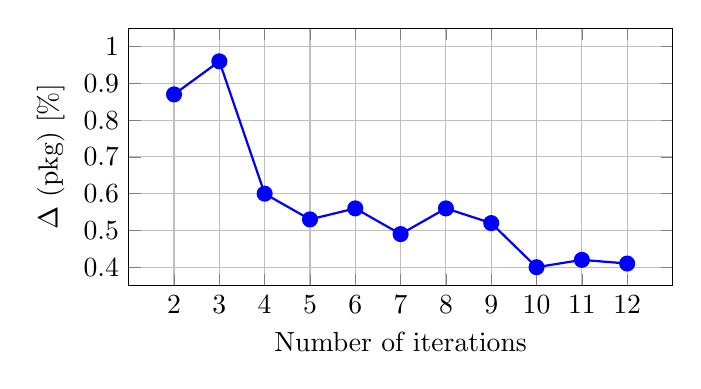
\begin{tikzpicture}
        \begin{axis}[
            width=0.7\textwidth,
            height=0.4\textwidth,
            xlabel={Number of iterations},
            ylabel={$\Delta$ (pkg) [\%]},
            xtick={2,3,4,5,6,7,8,9,10,11,12},
            ytick={0.2,0.3,0.4,0.5,0.6,0.7,0.8,0.9,1.0},
            ymin=0.35, ymax=1.05,
            grid=major,
            mark size=2.5pt,
            legend pos=north east
        ]
        \addplot[
            color=blue,
            mark=*,
            thick
        ] coordinates {
            (2,0.87)
            (3,0.96)
            (4,0.60)
            (5,0.53)
            (6,0.56)
            (7,0.49)
            (8,0.56)
            (9,0.52)
            (10,0.40)
            (11,0.42)
            (12,0.41)
        };
        \end{axis}
    \end{tikzpicture}
    \caption{Variation of results with respect to the number of benchmark iterations}
    \label{fig:number-benchmarks-graph}
\end{figure}


\begin{figure}[H]
    \centering
    \begin{tabular}{cc}
        \hline
        Number of iterations & $\Delta$ (pkg) \\
        \hline
        2  & 0.87\% \\
        3  & 0.96\% \\
        4  & 0.60\% \\
        5  & 0.50\% \\
        6  & 0.56\% \\
        7  & 0.49\% \\
        8  & 0.56\% \\
        9  & 0.52\% \\
        10 & 0.40\% \\
        11 & 0.42\% \\
        12 & 0.41\% \\
        \hline
    \end{tabular}

    \caption{Number of benchmarks for average calculation}
    \label{fig:number-benchmarks}
\end{figure}

\chapter{Scatter plot with python}
\label{chap:appendix-scatter-plot}

    \hypertarget{fig:conclusion-scatter-all}{} % anchor for links
\begin{figure}[h]
    \centering
    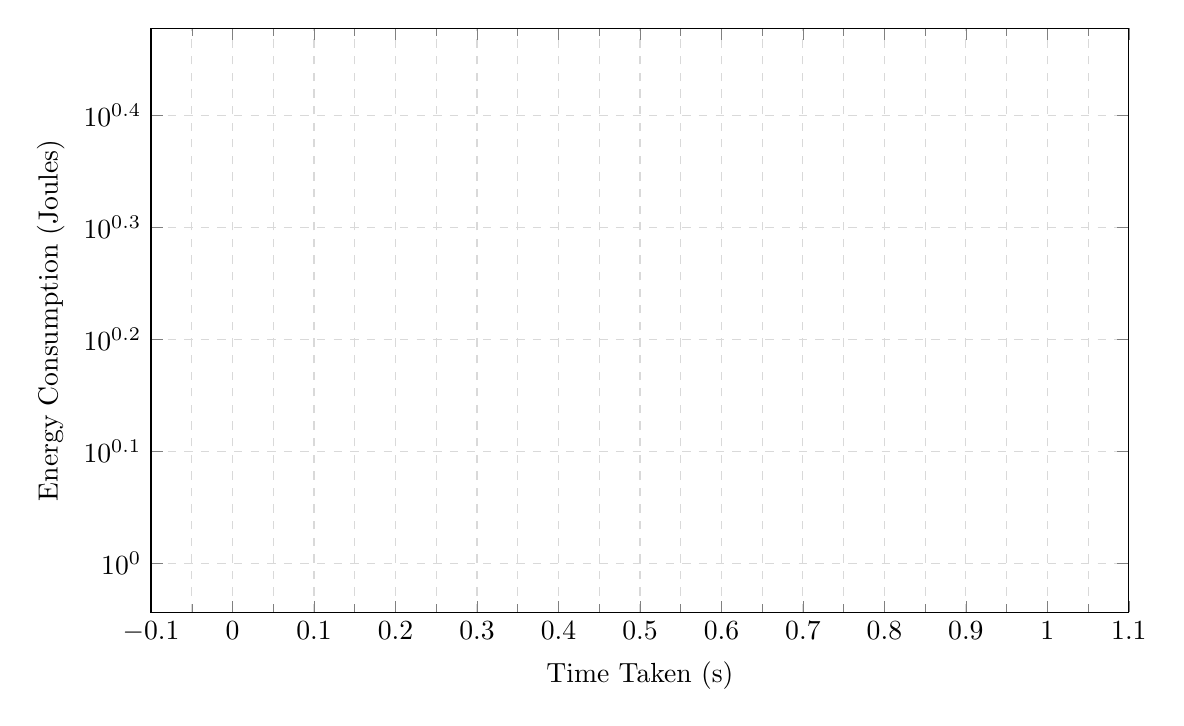
\begin{tikzpicture}
    \begin{axis}[
    width=14cm, height=9cm,
    xlabel={Time Taken (s)},
    ylabel={Energy Consumption (Joules)},
    ymode=log,
    grid=both, minor tick num=1,
    grid style={gray!30,dashed},
    legend style={at={(0.5,1.05)},anchor=south,legend columns=-1, draw=none},
    enlargelimits=0.1,
    clip=false
    ]
    % plots
    \PlotCXXconclusion
    \PlotPythonconclusion
    \PlotGoconclusion
    \PlotPyPyconclusion
    \legend{C++, Python, Go, PyPy}

    % clickable "button" inside the axis (top-right) → jump to no-Python figure
    \node[anchor=north east, fill=gray!15, draw, rounded corners,
      inner sep=3pt] at (axis description cs:0.98,0.98)
      {\hyperlink{fig:conclusion-scatter-nopy}{\shortstack{Show version \\ \emph{without} Python}}};


    \end{axis}
    \end{tikzpicture}
    \caption{All languages. Colors = language; labels = platform-cores.}
\end{figure}

\chapter{Declaration of Use of Generative AI}

\textbf{I have used Generative AI in this work} \quad \fbox{YES}

\section*{Part 1: Reflection on ethical and responsible behavior}

Keep in mind that the use of Generative AI entails risks and can have consequences that affect the moral integrity of your actions with it. Therefore, we ask you to answer the following questions honestly (mark what applies):

\textbf{1. In my interaction with Generative AI tools, I have submitted sensitive data with the proper authorization of the interested parties.}
\begin{itemize}
  \item[] \fbox{NO, I have not used sensitive data}
\end{itemize}

\textbf{2. I have submitted copyrighted materials with the proper authorization.}
\begin{itemize}
  \item[] \fbox{NO, I have not used protected materials}
\end{itemize}

\textbf{3. I have submitted personal data with the proper authorization of the interested parties.}
\begin{itemize}
  \item[] \fbox{NO, I have not used personal data}
\end{itemize}

\textbf{4. My use of the tool has respected the terms of use and ethical principles.}
\begin{itemize}
  \item[] \fbox{YES}
\end{itemize}


\section*{Part 2: Technical Use Declaration}


\subsection*{Documentation and writing}
I have used Generative AI for:
\begin{itemize}
  \item Search of bibliography to \href{https://www.google.com}{Google Scholar}, \href{https://openai.com}{GPT o3, o4}.
  \item Generation of tables based on provided data.
\end{itemize}

\subsection*{Development of specific content}
\begin{itemize}
  \item Programming assistance. \\
  I have asked for explanations of Python, Go and C++ code to \href{https://openai.com}{GPT 4o Copilot}, \href{https://www.anthropic.com/api}{Claude (3.5, 3.7, 4)}, \href{https://deepmind.google/models/gemini/pro/}{Gemini 2.5 Pro} and \href{https://qwenlm.github.io/}{Qwen 2.5}.

  \item Generation of elements. \\
  I have asked for generation of diagrams and tables based on benchmark data to \href{https://openai.com}{OpenAI's GPT 4.1, 4o, o4}, \href{https://deepmind.google/models/gemini/pro/}{Gemini 2.5 Pro}, \href{https://qwenlm.github.io/}{Qwen3} and \href{https://www.anthropic.com/api}{Claude (3.5, 4)}.

  \item Read proofing and correction of texts. \\
  I have asked for corrections of the text in the appendix and the main body of the work to \href{https://openai.com}{Gemini 2.5 Pro}.
\end{itemize}

\section*{Part 3: Reflection on Utility}

Please provide a personal assessment of the strengths and weaknesses you have identified in the use of Generative AI tools. Comment on whether it has helped you in the process of learning, development, or conclusions of the work.

The use of Generative AI tools has been beneficial in several ways. It has allowed me to quickly generate tables and diagrams based on benchmark data, which would have taken significantly more time to create manually and style consistently. Additionally, the ability to ask for explanations of code and receive immediate feedback has been invaluable in using new programming techniques.

I have not used AI to debug code as I have found out that by using AI to debug errors, it can lead to a lack of understanding of the underlying issues, and it can lead to an erroneous fix. 

In the process, I have learned also how LLMs work and what is the best way to use them, never accepting changes blindly, always checking the output.